
% Journal Article
% LaTeX Template
% Version 1.4 (15/5/16)
%
% This template has been downloaded from:
% http://www.LaTeXTemplates.com
%
% Original author:
% Frits Wenneker (http://www.howtotex.com) with extensive modifications by
% Vel (vel@LaTeXTemplates.com)
%
% License:
% CC BY-NC-SA 3.0 (http://creativecommons.org/licenses/by-nc-sa/3.0/)
%
%%%%%%%%%%%%%%%%%%%%%%%%%%%%%%%%%%%%%%%%%

%----------------------------------------------------------------------------------------
%	PACKAGES AND OTHER DOCUMENT CONFIGURATIONS
%----------------------------------------------------------------------------------------

\documentclass[twoside,twocolumn]{article}

\usepackage{blindtext} % Package to generate dummy text throughout this template

\usepackage[sc]{mathpazo} % Use the Palatino font
\usepackage[T1]{fontenc} % Use 8-bit encoding that has 256 glyphs
\linespread{1.05} % Line spacing - Palatino needs more space between lines
\usepackage{microtype} % Slightly tweak font spacing for aesthetics

\usepackage[english]{babel} % Language hyphenation and typographical rules

\usepackage[hmarginratio=1:1,top=32mm,columnsep=20pt]{geometry} % Document margins
\usepackage[hang, small,labelfont=bf,up,textfont=it,up]{caption} % Custom captions under/above floats in tables or figures
\usepackage{booktabs} % Horizontal rules in tables

\usepackage{lettrine} % The lettrine is the first enlarged letter at the beginning of the text

\usepackage{enumitem} % Customized lists
\setlist[itemize]{noitemsep} % Make itemize lists more compact

\usepackage{abstract} % Allows abstract customization
\renewcommand{\abstractnamefont}{\normalfont\bfseries} % Set the "Abstract" text to bold
\renewcommand{\abstracttextfont}{\normalfont\small\itshape} % Set the abstract itself to small italic text

\usepackage{titlesec} % Allows customization of titles
\renewcommand\thesection{\Roman{section}} % Roman numerals for the sections
\renewcommand\thesubsection{\arabic{subsection}} % roman numerals for subsections
\titleformat{\section}[block]{\large\scshape\centering}{\thesection.}{1em}{} % Change the look of the section titles
\titleformat{\subsection}[block]{\large}{\thesubsection.}{1em}{} % Change the look of the section titles

\usepackage{fancyhdr} % Headers and footers
\pagestyle{fancy} % All pages have headers and footers
\fancyhead{} % Blank out the default header
\fancyfoot{} % Blank out the default footer
\fancyhead[C]{Image Colorization $\bullet$ Sep 2019} % Custom header text
\fancyfoot[RO,LE]{\thepage} % Custom footer text

\usepackage{titling} % Customizing the title section

\usepackage{hyperref} % For hyperlinks in the PDF

\usepackage{longtable}

\usepackage{graphicx}

\usepackage{amsmath,amssymb}

\DeclareRobustCommand{\bbone}{\text{\usefont{U}{bbold}{m}{n}1}}

\DeclareMathOperator{\EX}{\mathbb{E}}% expected value

\usepackage{multicol}
\usepackage[table]{xcolor}



%----------------------------------------------------------------------------------------
%	TITLE SECTION
%----------------------------------------------------------------------------------------

\setlength{\droptitle}{-4\baselineskip} % Move the title up

\pretitle{\begin{center}\Huge\bfseries} % Article title formatting
\posttitle{\end{center}} % Article title closing formatting
\title{Automatic Image Colorization} % Article title
\author{%
\textsc{Tommaso Loss 1206692} \\
\textsc{Matteo Marcuzzo 1207249}
 \\[1ex] % Your name
\normalsize University of Padua \\ % Your institution
%\normalsize \href{mailto:john@smith.com}{john@smith.com} % Your email address
%\and % Uncomment if 2 authors are required, duplicate these 4 lines if more
%\textsc{Jane Smith}\thanks{Corresponding author} \\[1ex] % Second author's name
%\normalsize University of Utah \\ % Second author's institution
%\normalsize \href{mailto:jane@smith.com}{jane@smith.com} % Second author's email address
}
\date{\today} % Leave empty to omit a date
\renewcommand{\maketitlehookd}{%
\begin{abstract}
\noindent
In this report, we aim to explore some of the most recent advances in automatic image colorization of black and white pictures through the use of CNNs, as well as showcase our own implementation of one such. We describe the problem in its underconstrained nature, and discuss the approach by Zhang et al. \cite{Zhang:2016}, which was used as our main reference. We then proceed to exhibit our application and the results we obtained. Lastly, we briefly discuss some different approaches and architectures that have surfaced in recent years.
\end{abstract}
}

%----------------------------------------------------------------------------------------

\begin{document}

% Print the title
\maketitle

%----------------------------------------------------------------------------------------
%	ARTICLE CONTENTS
%----------------------------------------------------------------------------------------

\section{Introduction}

The task of colorizing grayscale images is not a simple one; to our imagination, some details might seem trivial (e.g. the sky is blue), yet some other are seemingly impossible to recover. As argued by Charpiat et al. \cite{Charpiat:2008}, color prediction is, in fact, inherently multimodal - meaning many objects can take several plausible colorizations, even without a significant change in shape. To convince ourselves of this, it suffices to think of a few examples. Apples, trees throughout seasons, artificial objects of various nature - a grayscale depiction of such has lost too much information for us to make a perfectly accurate guess. Nevertheless, we can easily imagine a \textit{plausible} colorization, and would like an automatic system to be able to do the same. 

Classical methods have either relied upon user input or a large repository of reference images to use at test time. Recent approaches, however, have successfully leveraged the developments of deep convolutional neural networks (CNNs) to obtain a solution that requires no database and is fast at test time \cite{Larsson:2016}.

The first and most important observation is that, in order to colorize images, a system must be able to interpret the semantic information of an image. In other words, it must be able to analyze the composition of the scene (what is in the picture) and where objects are located. Therefore, it comes as no surprise that CNNs are a perfect candidate for this task.

Furthermore, the task of colorization naturally fits a formulation where it is seen as a classification problem. In this, the classes to predict are a number of quantized color values (more on this later). Following the original authors' implementation \cite{Zhang:2016}, we produced a system that predicts color probabilities over 313 quantized color bins. These probabilities are then used at test time to produce the final colorization. The prediction itself is obtained by a single, feed forward pass through the network. 

A last observation is that, usually, not all colors are represented equally in a picture. It’s fairly common for backgrounds to have a grayish, desaturated color that accounts for a considerable part of the picture (e.g. cloudy skies, walls, dirt); consequently, a network trained on a large set of images will be biased towards these colors. As suggested by  \cite{Zhang:2016}, we introduce a form of \textit{class rebalancing} in our loss function to produce brighter colors, as well as push towards rarer ones.

\newpage


%------------------------------------------------

\section{Approach}
In this section, we discuss the theoretical approach to the problem. This includes a discussion on the preferred color space used for the data, the formulation of an appropriate loss function, the \textit{class rebalancing} solution to desaturated colors, the network architecture itself and the way its results are interpreted.


\subsection{Color space}
In the context of colorization as a classification task, usual color spaces such as RGB or BGR fall short. The main reason is quite simple; these would require a prediction over three different color channels. A common approach is to instead adopt the CIE-Lab color space (figure \ref{fig:cielab}), which restricts the problem to just two dimensions. This color space is also comprised of three channels, but has the useful characteristic that all grayscale information is stored in one of such. Indeed, the first channel (namely \textbf{L}) tracks the “lightness” value of a pixel (ranging from 0 for black to 100 for white). Channel \textbf{a} represents the color range between red and green, while channel \textbf{b} does the same for blue towards yellow. Furthermore, adopting this image representation technique makes it fairly trivial to obtain the black and white component of a picture, such that it might be used as input data (by simply discarding the \textbf{a} and \textbf{b} channels).

\begin{figure} [h]
	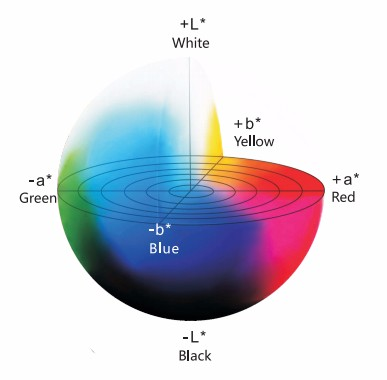
\includegraphics[width=\linewidth]{img/cielab.jpg}
	\caption{CIE-Lab color space}
	\label{fig:cielab}
\end{figure}

\subsection{Loss function}
As was briefly previewed, our system is geared to perform a classification task. In particular, its aim is to return probabilities over a set of color classes. One of the most common loss functions used in multinomial classification problems is that of \textit{Cross Entropy} (1), which calculates the average difference between the ground truth T and the predicted probability distribution P:

\begin{equation}
L_{cl}(P,T) = - \sum_{q} \: T_q \: log(P_q)
\end{equation}

This suits the task; however, in order to perform classification we first have to define the classes we want to predict. To this end, we synthesize the color space into a small number of \textbf{ab} pairs (with \textbf{L} = 50). A grid with space size 10 is overlaid onto the color space, thus reducing the number of relevant color pairs by a factor of ten. From the remaining colors, out of gamut ones are removed to obtain the final 313 color classes used in the classification task (figure \ref{fig:quantized}).


\begin{figure} [h]
	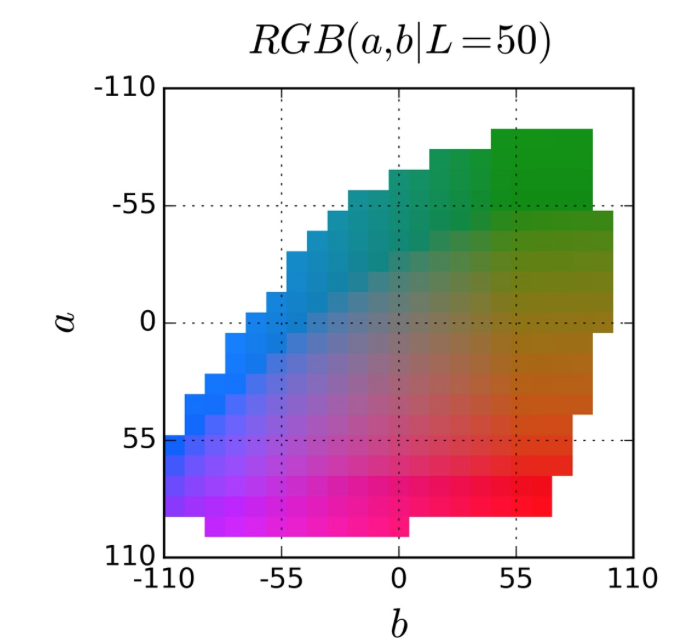
\includegraphics[width=\linewidth]{img/quantized.png}
	\caption{Quantized ab color space. Image credit:\cite{Zhang:2016}}
	\label{fig:quantized}
\end{figure}


In order to make a comparison, however, we now require ground truth values compatible to the predicted probabilities. The real color values are therefore transformed into probability distributions. This is achieved through \textit{soft-encoding}, by mapping each pixel color to its five nearest quantized \textbf{ab} color pairs. Each one is then attributed a weight based on the euclidean distance from the original color. Finally, these "distance-weights" are smoothed with a Gaussian kernel (with $\sigma=5$)\cite{Geoffrey:2015}.

However, that alone is not enough to obtain a meaningful colorization. This is because of the inherently uneven color distribution; in particular, background colors such as blue and green are much more prevalent than rare colors like purple. The resulting model will therefore be biased towards the most common colors, neglecting peculiar ones. 
The solution to this problem proposed by Zhang et al. \cite{Zhang:2016} is to recalibrate the probabilities by a factor \textit{v} based on the scarcity of the color. This process, named \textit{class rebalancing}, allows us to obtain our final loss formulation:

\begin{equation}
L_{cl}(P,T) = - \sum_{h,w}(v(T_{h,w}) \: \sum_{q} \: T_{h,w,q} \: log(P_{h,w,q}))
\end{equation}

\subsection{Class rebalancing}

The idea of class rebalancing is to take into account the inherent imbalance of class representation by reweighting the loss of each pixel at train time based on the pixel color rarity \cite{Zhang:2016}. The computation of these color weights starts off by calculating the number of occurrences of each \textbf{ab} color pair over the whole image dataset (mapping each pixel to its closest quantized bin). The resulting color frequencies are then turned into probability distributions, and subsequently smoothed with a gaussian kernel (much like was previously done with ground truth probabilities, $\sigma$ = 5). In order to soften the significant impact of these weights, these are mixed with a uniform probability distribution (p = 1/313). Finally, the reciprocal of the result is taken. This reverses the probability values, as our aim was for frequent colors to have small weights and vice-versa. The mixing factor $\lambda$ suggested by the original authors \cite{Zhang:2016} is of $1/2$. Furthermore, the result is normalized again, so that the weighting factor \textit{w} has a value of 1 on expectation.


\begin{equation}
w = (1 - \lambda)p + \frac{\lambda}{Q})^{-1}
\end{equation}

Where $p$ is the smoothed empirical distribution and $Q$ is the number of quantized bins (313). With regards to the previously discussed loss formulation (2), the weight $w$ of the most likely color is taken for $v$.

\subsection{Network architecture}

The network architecture we describe and implement follows the one proposed by Zhang et al.\cite{Zhang:2016}. Table \ref{tab:network} gives an overview of its structure and parameters. The network itself is comprised of 30 layers, which are either 2D convolutional layers or batch normalization layers.


\subsubsection{Layers}
The network is divided into 8 layer blocks, all of which are followed by a batch normalization layer. An exception is made for the last block, where a 1x1 conv and cross-entropy layer is imposed (the \textit{softmax} layer).

Each block contains 2 or 3 convolutional layers, all of which use a \textit{ReLU} activation function. In order to interpret the semantic information of an image, the network is required to learn a significant number of features. Therefore, the number of filters (correspondingly, the depth of the output volume) becomes quite large throughout the architecture, leading to a considerably high number of trainable parameters (around 25 million). Notably, we found that the authors' actual implementation \cite{Zhang:github} adopts an even greater number of filters, specifically in the last two blocks. Though we decided to adhere to the original formulation, our guess is that this change may have been an attempt to distinguish even finer features.

Batch normalization layers are applied after each convolutional block. This ensures that training may be performed with higher learning rates and with less worry with regards to the choice of initialization. In essence, the purpose of these layers is to normalize the activations of the previous layers at each batch, hence counteracting what is known as the \textit{internal covariate shift problem} - an issue caused by layers having activation distributions that are too different \cite{Sergey:2015}.

In regards to the spatial resolution of output, note how computational stride is used to downsample earlier blocks (namely, blocks 1 to 3). This is consistent with some recent studies \cite{Jost:2015}, which advise against the use of once popular pooling layers and instead suggest downsampling through larger stride when required. At the beginning of the last block, a 2D spatial upsampling is instead applied, effectively doubling the spatial resolution before the convolutional layers. 

Lastly, note the presence of dilated convolutions in blocks 5 and 6. This type of convolution has been shown to help in applications with dense predictions such as ours \cite{Fisher:2016}, since this approach to colorization is implemented as a classification problem for each pixel. At its core, what this approach allows us to do is to integrate information from different spatial scales much more aggressively,  forgoing the need to build a larger, multi-scale CNNs.


\begin{table*} [h!]
\centering
\captionof{table}{Network structure}
\setlength{\arrayrulewidth}{0.25mm}
\setlength{\tabcolsep}{15pt}
\renewcommand{\arraystretch}{1}
\begin{tabular}{|c|c|c|c|c|c|}

	\hline
	\rowcolor{gray!30}
	\textbf{Layer} & \textbf{Filters} & \textbf{Spac. Res.} & \textbf{Kernel size} & \textbf{Stride} & \textbf{Dilation}\\
	\hline
	\hline
	\multicolumn{6}{|c|}{input data (with size e.g. 224 * 224)}\\ \hline
	\rowcolor{gray!15}
	conv1\_1 & 64 & 224 & 3x3 & (1,1) & 1 \\ 
	conv1\_2 & 64 & 112 & 3x3 & (2,2) & 1 \\ \hline
	\multicolumn{6}{|c|}{Batch normalization}\\ \hline
	\rowcolor{gray!15}
	conv2\_1 & 128 & 112 & 3x3 & (1,1) & 1 \\ 
	conv2\_2 & 128 & 56 & 3x3 & (2,2) & 1 \\ \hline
	\multicolumn{6}{|c|}{Batch Normalization}\\ \hline
	\rowcolor{gray!15}
	conv3\_1 & 256 & 56 & 3x3 & (1,1) & 1 \\ 
	conv3\_2 & 256 & 56 & 3x3 & (1,1) & 1 \\ 
	\rowcolor{gray!15}
	conv3\_3 & 256 & 28 & 3x3 & (2,2) & 1 \\ \hline
	\multicolumn{6}{|c|}{Batch normalization}\\ \hline
	\rowcolor{gray!15}
	conv4\_1 & 512 & 28 & 3x3 & (1,1) & 1 \\ 
	conv4\_2 & 512 & 28 & 3x3 & (1,1) & 1 \\ 
	\rowcolor{gray!15}
	conv4\_3 & 512 & 28 & 3x3 & (1,1) & 1 \\ \hline
	\multicolumn{6}{|c|}{Batch normalization}\\ \hline
	\rowcolor{gray!15}
	conv5\_1 & 512 & 28 & 3x3 & (1,1) & 2 \\ 
	conv5\_2 & 512 & 28 & 3x3 & (1,1) & 2 \\ 
	\rowcolor{gray!15}
	conv5\_3 & 512 & 28 & 3x3 & (1,1) & 2 \\ \hline
	\multicolumn{6}{|c|}{Batch normalization}\\ \hline
	\rowcolor{gray!15}
	conv6\_1 & 512 & 28 & 3x3 & (1,1) & 2 \\ 
	conv6\_2 & 512 & 28 & 3x3 & (1,1) & 2 \\ 
	\rowcolor{gray!15}
	conv6\_3 & 512 & 28 & 3x3 & (1,1) & 2 \\ \hline
	\multicolumn{6}{|c|}{Batch normalization}\\ \hline
	\rowcolor{gray!15}
	conv7\_1 & 256 & 28 & 3x3 & (1,1) & 1 \\ 
	conv7\_2 & 256 & 28 & 3x3 & (1,1) & 1 \\ 
	\rowcolor{gray!15}
	conv7\_3 & 256 & 28 & 3x3 & (1,1) & 1 \\ \hline
	\multicolumn{6}{|c|}{Batch normalization}\\ \hline
	\multicolumn{6}{|c|}{2D Upsampling with size 2*2}\\ \hline
	\rowcolor{gray!15}
	conv8\_1 & 128 & 56 & 3x3 & (0.5,0.5)\footnotemark & 1 \\ 
	conv8\_2 & 128 & 56 & 3x3 & (1,1) & 1 \\ 
	\rowcolor{gray!15}
	conv8\_3 & 128 & 56 & 3x3 & (1,1) & 1 \\ \hline
	\multicolumn{6}{|c|}{Softmax Layer}\\ \hline

\end{tabular}
\label{tab:network}
\end{table*}



\subsubsection{Layer parameters}

All convolutional layers have their weights initialized through \textit{He Normal} \cite{Kaiming:2015} initialization. This method initializes weights randomly, while also taking into consideration the size of the previous layer, which helps in attaining a controlled initialization. As a consequence, the result is a faster and more efficient gradient descent. In practice, samples are drawn from a truncated normal distribution centred on 0, and with $stddev=\sqrt{(2/fan\_in)}$, where $fan\_in$ is the number of incoming neurons.

This type of initialization also agrees with the choice of using \textit{ReLU} activation functions, as it was designed with such an activation unit in mind. We apply an \textit{L2} regularization function to the kernel matrix in all layers, which constrains the optimisation algorithm in an attempt to minimize overfitting:

\begin{equation}
Loss = Error(y,\tilde{y}) + \lambda\sum_{i=1}^{N} w_i^2
\end{equation}

All layers utilise a padding of type ‘\textit{same}’, meaning the layer’s output have the same spatial dimension as the outputs (this is achieved through \textit{0-padding}).

\subsubsection{Optimizer}
Our choice for optimizer was that of \textit{Adam} (derived from \textit{Adaptive Moment Estimation}) \cite{Diaderik:2015}. While we initially experimented using SGD (Stochastic Gradient Descent), we found that \textit{Adam} gave us the best results in the scope of our experiments. That is, when considering the restricted nature of our resources, we consider Adam to be the better choice, though recent discoveries demonstrate this optimizer to generalize poorly in the long run \cite{Nitish:2017}.


\subsection{Prediction evaluation}

Once the model has been trained, prediction is done through a single, feed forward pass through the network, which only retains the \textbf{L} channel of input pictures and produces a probability distribution over the 313 quantized colors for each pixel.

It remains to decide how to use this information to produce our colorization. One choice is to take the most frequent and probable values; while this idea results very vibrant colors, it often produces spatially inconsistent results and “hard transitions” from one color to the other. A better approach could therefore be to take the mean over each of the quantized bins, weighing them by their probability. This ensures softer transitions, but runs into the unwanted consequence that colors become desaturated, as too much importance is attributed to lower probability colors.

The solution proposed in \cite{Zhang:2016} attempts to have the best of both worlds. The authors suggest taking what they name the “\textit{annealed mean}” of the distribution. This consists of an interpolation of the softmax distribution by means of a temperature value T, and consequently taking the mean of the result (6). Strictly speaking, this implies that each value is divided by the aforementioned temperature, whose value ranges from 0 to 1 (the suggested value is 0.38, which we adhered to). This ensures that more importance is given to high probability values, resulting into the vibrant colorization desired as well as better spatial consistency.

\footnotetext{The .5 stride is simulated through a 2d upsampling operation. Earlier implementations made instead use of a deconvolutional layer, but we found this other approach to work better in practice.}

\begin{equation}
H(P) = \EX[f(P)]
\end{equation}

\begin{equation}
f(P) = \frac{\exp(log(P)/T)}{\sum_q \: \exp(log(P_q)/T)}
\end{equation}

%------------------------------------------------
\newpage

\section{Experimentation}
In this section, we discuss the actual implementation and the results of our experiments. This includes an overview of languages and libraries used, as well as some insights about actual code. We then go on to discuss the finer details of our experiments, such as data utilized, hyperparameters tested and hardware specifications. Finally, we present our results, giving our thoughts in regards to error and metric values.

\subsection{Implementation}

The full implementation was written to work with \texttt{Python 2.7}, and is based on \texttt{Tensorflow 1.14} and \texttt{Keras}. While we initially set out to create a model purely in \texttt{Tensorflow}, we soon realized that \texttt{Keras} was the better option, as it allowed us to work in a simpler yet more efficient fashion.

Since the data required quite a bit of preprocessing, the loading of images from file as well as the creation of batches is handled by a custom class, \texttt{DataGenSequence}. Through this, the system may load any color image of a given format and generate training data by stripping it of its \textbf{ab} channels, as well as generating a ground truth through a \textit{soft-encoding} method, namely \texttt{get\_soft\_encoding}.

This allows for extra flexibility, as images may be resized and converted in format at run time. While we realize that larger datasets would most certainly benefit in storing the preprocessed data for efficiency reasons, we often encountered the need to make changes to our training data (i.e. swapping between datasets as well as image sizes) due to our computational constraints. Thus, our implementation was mostly intended to simplify our tests.

\begin{figure} [h]
	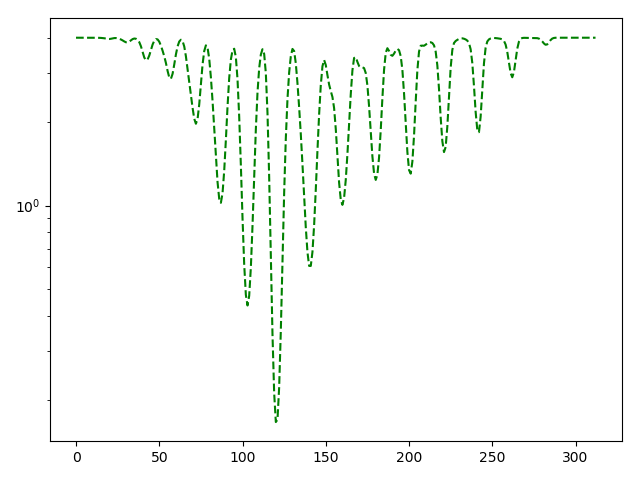
\includegraphics[width=\linewidth]{img/ours.png}
	\caption{Prior probability of quantized colors, as calculated on our dataset}
	\label{fig:oursprior}
\end{figure}

\begin{figure} [h]
	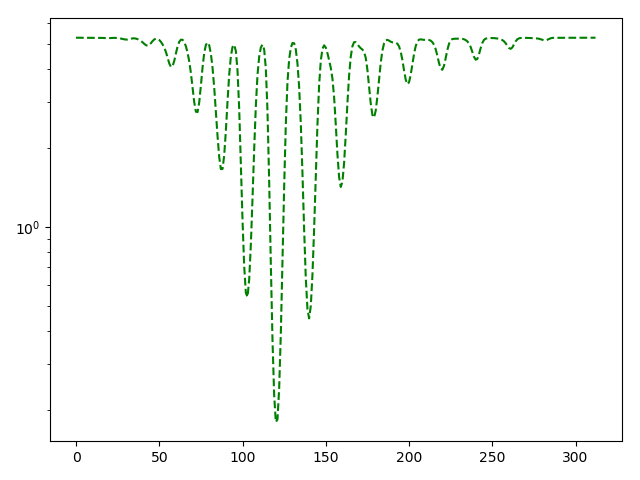
\includegraphics[width=\linewidth]{img/zhang.png}
	\caption{Zhang et al. \cite{Zhang:github}'s prior probability results}
	\label{fig:zhangprior}
\end{figure}

\subsection{Dataset}

While we initially planned on using the full Image Net dataset \cite{Imagenet}, we soon realized we lacked the computational power to process it in its full size, even after we decided to move our experiments on the Google Cloud Platform \cite{GCP} (more on this later). We therefore decided on a suitable subset, which we increased from time to time as we gained confidence in the correctness of our implementation. Our final dataset contains 175’333 images (roughly 20gb worth of pictures) randomly and evenly selected from the 2017 Large Scale Visual Recognition Challenge Image Net dataset \cite{ImNetChallenge:2017}. Of this, 99\% was used as a training set, while the remaining 1\% for validation. While these percentages might seem odd, we found many implementations used even less images for validation. The authors \cite{Zhang:2016} themselves utilize a dedicated validation set of 10k images, over the 1.3M used for their training. In our experience, we found that our proposed value presented the least discrepancy overall between the values of loss and validation loss, while still allowing validation to be performed in a timely manner.


Some remarks need to be made with regards to the prior color probability of the dataset (used in the class rebalancing method). While we did write our own implementation and initially used it, our final version utilizes the results as calculated by Zhang et al. \cite{Zhang:2016}, which are publicly available \cite{Zhang:github}. Due to our limited resources, we could only manage to calculate such prior on either a small subset of our dataset or on greatly downscaled images. It is worth mentioning that, if we make a comparison, our prior factor (figure \ref{fig:oursprior}) does not differ greatly from the original authors’ (figure \ref{fig:zhangprior}). We decided nonetheless to utilize the more accurate data, as it is based on the full Image Net dataset.

\subsection{Hyperparameters}

Once we finalized our implementation, we worked on tuning some of the main hyperparameters, mainly so that we could find the values that best suited the reduced scale of our experiments. 

\subsubsection{Image size}
Unsurprisingly, our experiments show that using higher image sizes results in better training. Our earlier tests used smaller images in order to hasten the process and fit in the limited memory of our local machines, but with our eventual move to the cloud we settled on a size of 256x256 pixels. This allowed to retain a good amount of detail while maintaining a batch size we were comfortable with.

\subsubsection{Batch size}
Though we tried a few different sizes for the data batches to be used at each training step, we settled on a value of 64. This pushed the limits of our hardware to its maximum (with each batch utilizing almost the full 15GB of GPU memory available in our latest virtual machine). While we tried to vary the size of images to be able to create larger batches, we found this compromise to be what gave us the best results. This may quite obviously be because of the higher definition of the images, but recent works also advise against using larger and larger batches \cite{Nitish:2017}, which is something we took into consideration.

\subsubsection{Learning rate}
We tested various learning rates, and settled on a value of  3.16e-5 (again, using the \textit{Adam} optimizer). Many values were experimented with, but we found that higher orders of magnitude would quickly become stuck after a rapid descent. Anything significantly lower, on the other hard, would have too much of a hard time exiting points of local optimum.
The final chosen value allows for training to be fast in the beginning without exhibiting wild swings in the behaviour of the loss value in its later epochs.


\subsection{Hardware details}

The following are the hardware specifics for the machines used in our tests. We performed initial tests and training on one of our home machines, the details of which are as follows:
\begin{itemize}
\item \textbf{CPU}: AMD Ryzen 5 1600x  6-core (3.6GHz);
\item \textbf{GPU}: NVIDIA GeForce GTX 970 (4 GB GDDR5);
\item \textbf{Memory}: 16 GB DDR4;
\item \textbf{Persistency}: 500GB Force MP510 M.2 SSD;
\item \textbf{OS}: Windows 10 Enterprise.
\end{itemize}

The aforementioned hardware allowed us to work on small datasets and downsized images, but in the long run did not have the GPU capabilities necessary for our needs, even on a reduced scale. Namely, we required a considerable upgrade in GPU memory in order to work on bigger images as well as larger batches. We therefore decided to move our experiments on the Google Cloud Platform \cite{GCP}, where we instantiated a virtual machine with the following specifications:
\\
\\

\begin{itemize}
	\item \textbf{vCPU}: 4 virtual cores;
	\item \textbf{GPU}: NVIDIA Tesla P4 (8 GB GDDR5) / T4 (16 GB GDDR6) (later tests);
	\item \textbf{Memory}: 15GB RAM;
	\item \textbf{Persistency}: 65 GB standard persistent disk (HDD);
	\item \textbf{OS}: Ubuntu 18.10.
\end{itemize}

As stated above, we initially performed training on an NVIDIA Tesla P4 GPU, but later decided to upgrade to the T4 because of its higher memory capacity.


\subsection{Performance and results}

What follows is a brief overview of our experimental outcomes. This includes metrics considered, an analysis of loss value trends, a recount of our most significant training runs and finally a showcase of our results.

\subsubsection{Metrics}
As the original authors claim \cite{Zhang:2016}, evaluating the quality of synthesized images is a difficult task in itself. Common qualitative metrics, such as RMS error on pixel values, fail to capture the notion of visual realism, which is what the system is instead trying to achieve.
One could nonetheless measure the raw prediction accuracy (L2 distance from the ground truth in the \textbf{ab} color space), but we decided against this as it does not reflect the true aim of the system (that of a plausible colorization). In fact, Zhang et al. \cite{Zhang:2016} show that a metric of the sort would give a rather good score even for an image fully colorized in gray, which is not ideal.

As a result, the best way to verify the quality of the result is to perform a test on human subjects. While the scope of our experiments is nowhere near as rigorous as the referenced counterpart, we thought it would be interesting to put the results of our model to use by attempting our own version of the proposed tests.

We asked fifteen partecipants to identify real images given a choice between our colorized version of a picture and its original. Each pair of pictures was shown for five seconds and 20 pairs were shown in total.
Figure \ref{fig:testres} summarizes the results. The highest number of mistakes made is 50\% (as if all the choices were made randomly between two equally realistic images), whereas the best achieving subjects managed to have an error rate of 0\%. Our average fooling percentage is 30\%, which resembles the original authors' result of 32\%.

Of course, we do not claim any scientific validity to our test, as the subject pool was far too small to prove of any significance. Nonetheless, the results are at least promising, and provide some positive feedback on the goodness of the model.

\begin{figure}
	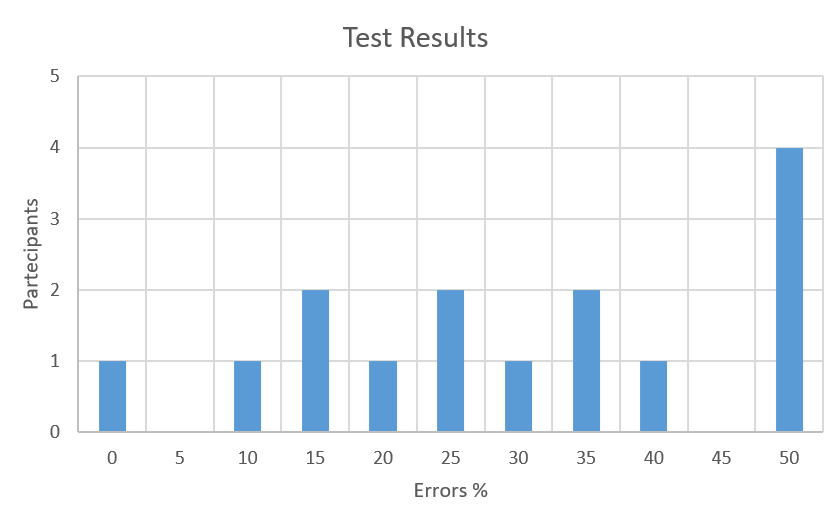
\includegraphics[width=\linewidth]{img/graficotest.png}
	\caption{Human "fooling" test results}
	\label{fig:testres}
\end{figure}

\subsubsection{Loss}

As just claimed, commonly used metrics are difficult to apply to a problem of this kind, as the objective of the system is to produce a subjectively \textit{plausible} result.
Therefore, while it may seem unsatisfactory in some ways, one has to rely on a pure analysis of loss values throughout training epochs. As a reminder, this value represents the mean difference between the predicted probability distribution of colors and the actual distribution obtained through soft encoding of the ground truth.

Empirically speaking, we found that the system first produces some promising results when validation loss falls below a value of 5, when it gains the confidence to attempt some vivid colorizations. In earlier epochs, resulting pictures are still desaturated and grayish. Learning slows massively around the value of 4, where it begins a slow descent. In later epochs, the system becomes more adept at recognizing shapes and coloring them correctly. As one would expected, we find that a good indicator of how well training is proceeding is how consistent the value of loss in training is with its validation counterpart. 

\subsubsection{Training runs}

Figure \ref{fig:loss} and \ref{fig:valloss} display the change in loss on the training and validation set throughout various epochs. These graphs refer to our latest training session, performed on our full 20gb dataset on an NVIDIA Tesla T4. The test ran for almost 67 hours, after which we decided to stop the instance as we began to see no improvement. Correspondingly, later models struggled to improve on validation loss, and appeared to be overfitting on certain color patterns.


Our latest run was by far our longest, while previous tests were mostly aimed at finding a good balance between our hyperparameters. Our experimental results confirm the well known fact that smaller datasets provide insufficient information to the network. Practically speaking, we noted that with less images given to the network the loss value would converge much faster and at higher values, and would thereon be unable to improve. Furthermore, a gap between training and validation loss would quickly appear, with the latter getting stuck at higher values (a clear indication of overfitting on training data). 

Conversely, figures \ref{fig:loss} and \ref{fig:valloss} show the benefit of bigger datasets, with the two curves being much more consistent with one another throughout training.


\begin{figure}[h]
	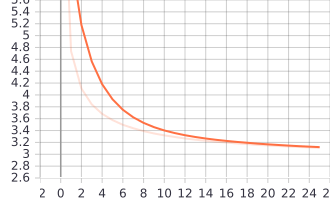
\includegraphics[width=\linewidth]{img/loss.png}
	\caption{Loss, smoothing=0.6}
	\label{fig:loss}
\end{figure}

\begin{figure}[h]
	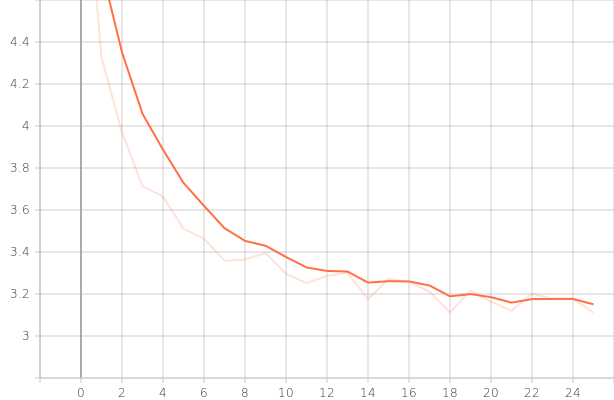
\includegraphics[width=\linewidth]{img/val_loss.png}
	\caption{Validation Loss, smoothing=0.6}
	\label{fig:valloss}
\end{figure}

\subsubsection{Results}

Figure \ref{fig:bestimgs} shows some of what we consider the best results of our network. Most importantly, some of these pictures display particularly vivid colors, thanks to the implementation of the class-rebalanced loss function. Furthermore, note how figure \ref{fig:banio} exemplifies the multimodal nature of colorization; both images seem plausible, yet the colors are quite distinct from one another.

Figure \ref{fig:bad} shows some failure cases. Unsurprisingly, we noticed that our system struggles with objects with great amount of details. We hypothesize this to be a direct consequence of the lack of data, as well as the need for a more refined architecture, ideally able to handle larger and more detailed images.

\begin{figure}
	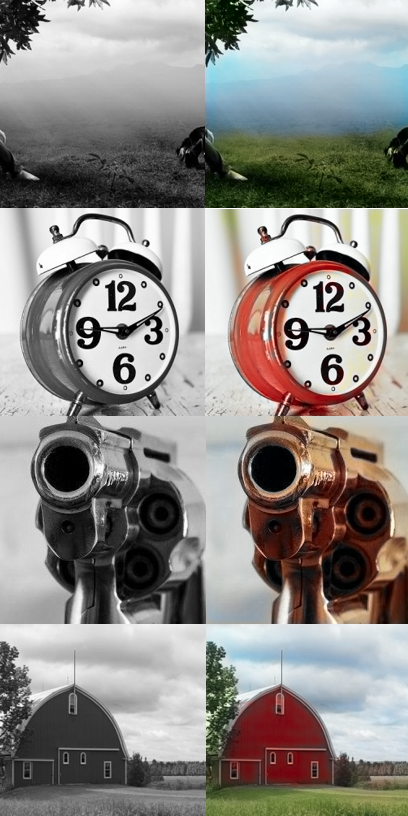
\includegraphics[width=\linewidth]{img/bestimgs.png}
	\caption{A sample of our best colorizations}
	\label{fig:bestimgs}
\end{figure}

\begin{figure}
	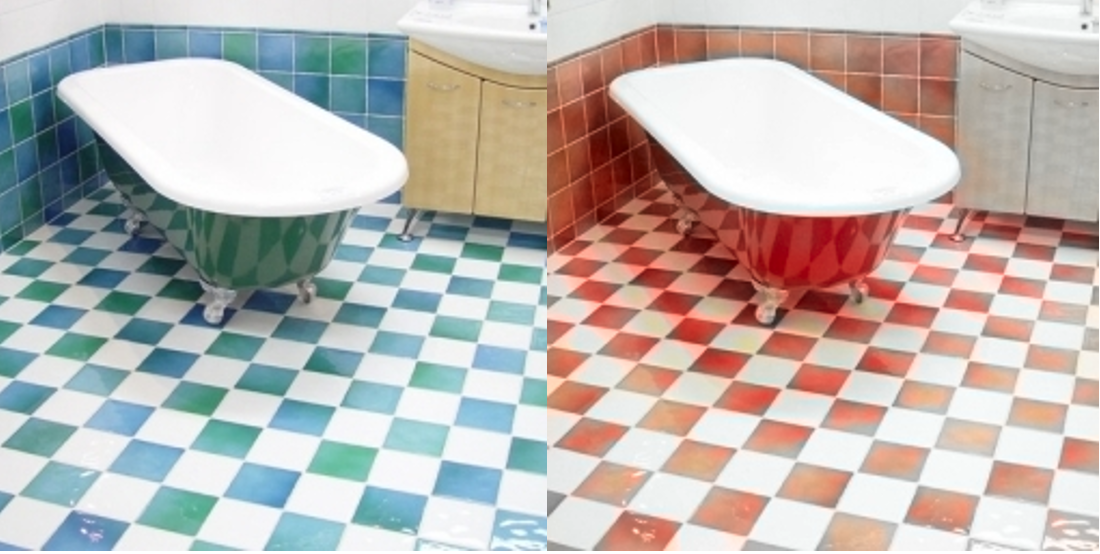
\includegraphics[width=\linewidth]{img/banio.png}
	\caption{To the left, the original image; \\ To the right, our colorization}
	\label{fig:banio}
\end{figure}

\begin{figure}
	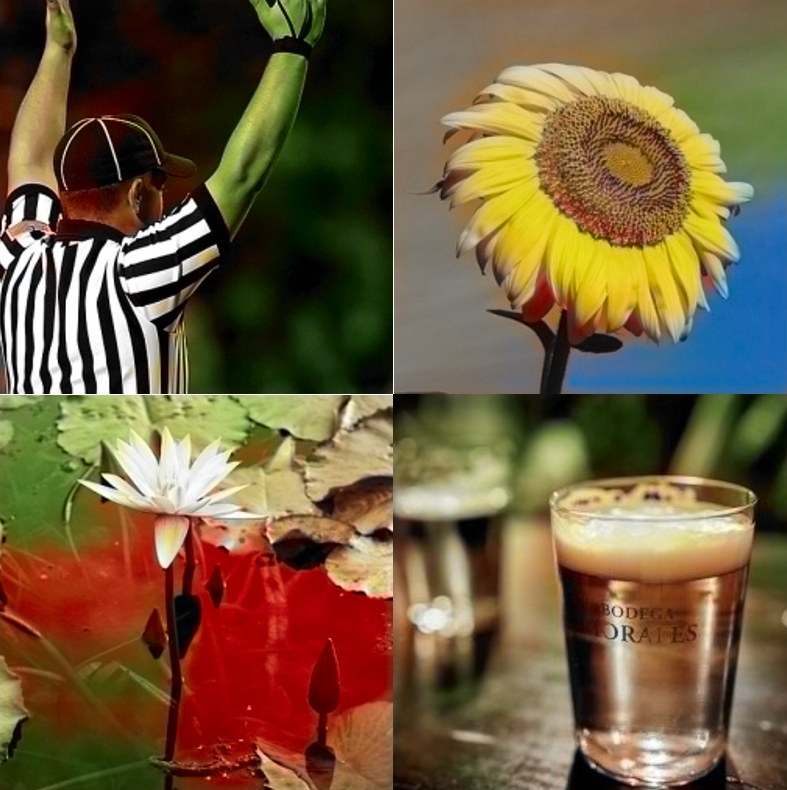
\includegraphics[width=\linewidth]{img/bad.png}
	\caption{Unsuccessful colorizations from out network}
	\label{fig:bad}
\end{figure}

\subsection{Final considerations}

We conclude this chapter by making some considerations and comparisons with the original authors’ version \cite{Zhang:2016}.

First and foremost, when taking into account the restricted scale of our experiments, we are quite happy with the results obtained. The referenced implementation utilizes the Caffe framework, which at times made it difficult to compare some of the finer details of the network. As mentioned, the version they make available \cite{Zhang:github} was slightly adapted to be able to better detect finer features; we refrained from such adaptations, as they would have slowed our training sessions significantly without necessarily resulting in better performance.

Undoubtedly, the authors had access to much more powerful computational hardware, which allowed them to work with better detailed images as well as more data (the entirety of Image Net \cite{Imagenet}). Nonetheless, the core of the implementation remains the same. The network in itself is quite deep, which is reflected by lengthy training times. While we did try many different betterments for the architecture in itself (performing the same operations, but in different ways), at this point in time we firmly believe that our best bet for any improvement is to simply utilize more data.

Lastly, we note a few interesting and practical uses that a system such as this has been shown to have. The representation learned by this network, though aimed towards colorization, has been proven useful for tasks that are likewise geared towards the detection of semantic information. Some examples include object classification, detection and segmentation \cite{Zhang:2016}.


%------------------------------------------------

\newpage

\section{Recent developments}

In this section, we propose a brief insight on recent developments in the use of Deep Neural Networks for the task of image colorization.

\subsection{User-guided image colorization}
Expanding upon their previous work, the authors of our main reference paper recently continued their work and proposed a new architecture for the task of colorization \cite{Zhang:2017}. In this case, however, the authors embrace the uncertain nature of the task and suggest that better colorization may be achieved through sparse and limited user input. This allows for real time correction of mistaken colors as well as the possibility to create custom colorizations.

The architecture proposed is similar to their previous, but is expanded upon. In fact, the number of conv-ReLU layer blocks is increased to 10, with the first 8 blocks maintaining the same architecture as before. Furthermore, these shared blocks utilize pre-trained weights from their previous experiments \cite{Zhang:2016}, which are then fine tuned during training. The added blocks are trained from scratch, and symmetric shortcut connections are added to help the network recover spatial information (not unlike what happens in a \textit{U-net} architecture).

We also note the presence of smaller, auxiliary networks, though we skip their discussion as they are only present to provide color suggestions to the user.


\subsection{Colorization with self-attentive Generative Adversarial Networks}

In his openly available work \textit{DeOldify} \cite{Jason:github}, software engineer Jason Antic shows an interesting use of self-attention mechanisms and GANs to achieve more precise colorization, as well as displaying some outstanding results in video colorization.

Self-attention mechanisms \cite{Ashish:2017}, which have been shown to produce state-of-the-art results in the field natural language processing, have recently provided good results in image-related tasks. At their essence, self attention mechanisms provide a way to model long-range dependencies between sections of an image. In other words, while convolutional networks focus on relative location and proximity, attention is able grab contextual information from distant image regions \cite{Chris:guide}; intuitively, this makes the two complementary in nature.

On the other hand, the framework of Generative Adversarial Networks (GANs) provides a novel way  to approach unsupervised learning in a manner that closely resembles game theory \cite{Ian:2014}. This framework is comprised of two networks: a \textit{generator}, which acts much like our network would, and a \textit{discriminator}, which receives data from both the ground truth and the generator. The task of the discriminator is to predict whether the data is true or artificial. The generator’s objective therefore becomes to maximise the probability that the discriminator is “fooled”, in the sense that it accepts data from the generator as true data.

Very recent works combine these two approaches \cite{Han:2019}, claiming that self-attention can help the generator to recognize finer details as well as allowing the discriminator to more accurately enforce geometric constraints on the global image.

While the original paper that introduced the idea of Self-attentive Generative Adversarial Networks did so with regards to an image generation task, the author of \textit{DeOldify} demonstrates that it suits the colorization task very well. Interestingly enough, the model used for the generator network follows a \textit{U-Net} architecture, much like Zhang et al.\cite{Zhang:2017} in their most recent work.

%------------------------------------------------

\newpage
\onecolumn
\section{Conclusions}

In this report, we tackled the task of image colorization through the use of Deep Neural Networks. We showcased an approach that produces fair, automatic colorization by treating the colorization task as a classification problem. We discussed the advantages of using the CIELAB color space, as well as introducing the \textit{class rebalancing} method to enhance the representation of rare colors. We then proceeded to combine all this information with the CNN architecture proposed by Zhang et al. \cite{Zhang:2016} and produced our own Tensorflow implementation of such.

Considering our novice state with regards to the world of deep learning, we are satisfied with the results obtained. Much of our time was spent learning the Tensorflow framework as well as tinkering with many of the finer details (such as image preprocessing and proper handling of tensors). Furthermore, we were forced by the computational necessities of the task to migrate our work on the Google Cloud Platform \cite{GCP}, which proved challenging but rewarding.

All things considered, image colorization - much like many image related tasks - is difficult. Though we argued for specific issues such as the multimodal nature of colors, much of this difficulty comes from the inherent necessity for big data. Images in themselves are a particularly rich medium of information, which further amplifies these computational challenges.

Works on this particular topic are very recent, and as such improvements are being published every passing year. We concluded by showcasing some of the latest developments in the field, which bring thrilling results to the table. We are excited to see how these innovative architectures will further advance in the future.   

%------------------------------------------------

%----------------------------------------------------------------------------------------
%	REFERENCE LIST
%----------------------------------------------------------------------------------------
\newpage
\twocolumn
\clearpage

\begin{thebibliography}{99} % Bibliography - this is intentionally simple in this template



\bibitem[1]{Zhang:2016}
Richard Zhang, Phillip Isola, Alexei A. Efros (2016).
\newblock Colorful Image Colorization.

\bibitem[2]{Charpiat:2008}
Charpiat, G., Hofmann, M., Scholkopf, B. (2008).
\newblock Automatic image colorization via multimodal
predictions.
\newblock Computer Vision-ECCV 2008. Springer 126 - 139

\bibitem[3]{Larsson:2016}
Larsson, G., Maire, M., Shakhnarovich, G. (2016).
\newblock Learning representations for automatic
colorization.
\newblock European Conference on Computer Vision (2016)

\bibitem[4]{Geoffrey:2015}
Geoffrey Hinton, Oriol Vinyals, Jeff Dean (2015)
\newblock Distilling the Knowledge in a Neural Network

\bibitem[5]{Sergey:2015}
Sergey Ioffe, Christian Szegedy (2015).
\newblock Batch Normalization: Accelerating Deep Network Training by Reducing Internal Covariate Shift.

\bibitem[6]{Jost:2015}
Jost Tobias Springenberg, Alexey Dosovitskiy, Thomas Brox, Martin Riedmiller (2015).
\newblock Striving for simplicity: the all convolutional net.

\bibitem[7]{Fisher:2016}
Fisher Yu, Vladlen Koltun (2016).
\newblock Multi-scale context aggregation by dilated convolutions.

\bibitem[8]{Kaiming:2015}
Kaiming He, Xiangyu Zhang, Shaoqing Ren, Jian Sun (2015).
\newblock Delving Deep into Rectifiers: Surpassing Human-Level Performance on ImageNet Classification.

\bibitem[9]{Diaderik:2015}
Diederik P. Kingma, Jimmy Lei Ba (2015).
\newblock Adam: A Method for Stochastic Optimization.

\bibitem[10]{Nitish:2017}
Nitish Shirish Keskar, Richard Socher (2017).
\newblock Improving Generalization Performance by Switching from Adam to SGD.

\bibitem[11]{Imagenet}
Imagenet.
\newblock \href{http://www.image-net.org/index}{ImageNet home page}.

\bibitem[12]{ImNetChallenge:2017}
Imagenet Large Scale Visual Recognition Challenge (2017).
\newblock \href{http://www.image-net.org/challenges/LSVRC/}{Imagenet challenge page}.

\bibitem[13]{GCP}
Google Cloud Platform.
\newblock \href{https://cloud.google.com/}{Google Cloud home page}.

\bibitem[14]{Nitish:2017}
Nitish Shirish Keskar, Dheevatsa Mudigere, Jorge Nocedal, Mikhail Smelyanskiy, Ping Tak Peter Tang (2017).
\newblock On large-batch training for deep learning: generalization gap and sharp minima.

\bibitem[15]{Zhang:github}
Richard Zhang, Phillip Isola, Alexei A. Efros.
\newblock \href{https://github.com/richzhang/colorization}{Repository}.

\bibitem[16]{Zhang:2017}
Richard Zhang, Jun-Yan Zhu, Phillip Isola, Zinyang Geng, Angela S. Lin, Tianhe Yu, Alexei A. Efros (2017).
\newblock Real-Time User-Guided Image Colorization with Learned Deep Priors.

\bibitem[17]{Jason:github}
Jason Antic.
\newblock \href{https://github.com/jantic/DeOldify}{DeOldify repository}

\bibitem[18]{Ashish:2017}
Ashish Vaswani, Noam Shazeer, Niki Parmar, Jakob Uszkoreit, Llion Jones, Aidan N. Gomez, Lukasz Kaiser, Illia Polosukhin (2017).
\newblock Attention Is All You Need.

\bibitem[19]{Chris:guide}
Chris Nicholson.
\newblock \href{https://skymind.ai/wiki/attention-mechanism-memory-network}{A Beginner's Guide to Attention Mechanisms and Memory Networks}

\bibitem[20]{Ian:2014}
Ian J. Goodfellow, Jean Pouget-Abadie, Mehdi Mirza, Bing Xu, David Warde-Farley,
Sherjil Ozair, Aaron Courville, Yoshua Bengio (2014).
\newblock Generative Adversarial Nets.

\bibitem[21]{Han:2019}
Han Zhang, Ian Goodfellow, Dimitris Metaxas, Augustus Odena (2019).
\newblock Self-Attention Generative Adversarial Networks.



\end{thebibliography}

%----------------------------------------------------------------------------------------

\end{document}
